% $HeadURL: https://sbgn.svn.sourceforge.net/svnroot/sbgn/trunk/documents/specifications/EntityRelationship/Level1/sources/tag.tex $

\color{red}

\subsection{Glyph: \glyph{Tag}}
\label{sec:tag}

A \glyph{tag} is a named handle, or reference, to another EN (\sect{ENs}) or a container node (\sect{CNs}).  \glyph{Tags} can be used to identify elements in SBGN \glyph{submaps} (\sect{submap}).

\begin{glyphDescription}

\glyphSboTerm Not applicable.

\glyphContainer A \glyph{tag} is represented by a rectangle fused to an empty arrowhead, as illustrated in \fig{tag}.  The symbol should only be linked to one and only one edge (\ie it should reference only one EN or container).

\glyphLabel A \glyph{tag} is identified by a label placed in an unbordered box containing a string of characters.  The characters can be distributed on several lines to improve readability, although this is not mandatory.  The label box must be attached to the center of the container.  The label may spill outside of the container.

\glyphAux A \glyph{tag} does not carry any auxiliary items. 

\end{glyphDescription}

\begin{figure}[H]
  \centering
  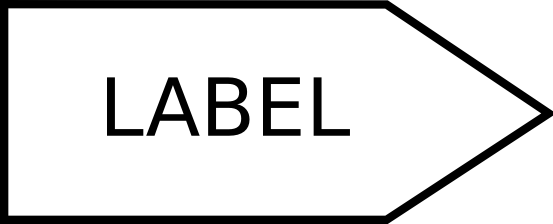
\includegraphics[scale = 0.3]{images/tag}
  \caption{The \ER glyph for \glyph{tag}.}
  \label{fig:tag}
\end{figure}

\normalcolor

% The following is for [X]Emacs users.   Please leave in place.
% Local Variables:
% TeX-master: "../sbgn_ER-level1"
% End:

